\documentclass[10pt, a4paper]{article}
\usepackage[paper=a4paper, left=1.5cm, right=1.5cm, bottom=1.5cm, top=3.5cm]{geometry}
\usepackage[T1]{fontenc}
\usepackage[spanish]{babel}
\usepackage[utf8]{inputenc}
\usepackage{indentfirst}
\usepackage{fancyhdr}
\usepackage{a4wide}
\usepackage[dvipsnames,usenames]{color}
\usepackage{float}
\usepackage{amsmath}
\usepackage{listings}
\usepackage{listingsutf8}
\usepackage{graphicx}
\usepackage{amsfonts}
\usepackage{verbatim}
\usepackage{latexsym}
\usepackage{lastpage}
\usepackage[colorlinks=true, linkcolor=blue]{hyperref}
\usepackage{calc}

\newcommand{\f}[1]{\text{#1}}
\newcommand{\real}{\mathbb{R}}
\newcommand{\nat}{\mathbb{N}}
\newcommand{\eme}{\mathcal{M}}
\newcommand{\emeh}{\widehat{\mathcal{M}}}
\newcommand{\ere}{\mathcal{R}}

\sloppy

\setlength{\voffset}{-0.5cm}
\setlength{\hoffset}{0.7cm}
\setlength{\headsep}{0pt}
\setlength{\headheight}{0pt}
\setlength{\oddsidemargin}{-0.7in}
\setlength{\marginparwidth}{-0.5cm}
\setlength{\textwidth}{18cm}
\setlength{\footskip}{2pt}
\setlength{\topmargin}{0in}
\setlength{\textheight}{25cm}
\setlength{\fboxrule}{3pt}

\begin{document}
\thispagestyle{empty}
\begin{center}

\Huge{ \bf{UNIVERSIDAD DE BUENOS AIRES}}
\\
\LARGE{\bf{Facultad de Ciencias Exactas y Naturales}}
\\
\textbf{Departamento de Computaci\'on}
\\
\textbf{Organizaci\'on del Computador}
\vspace{2.0\baselineskip}
\end{center}


\begin{figure}[h] %[h] Aqui [b] para button [t] para top
\begin{center}

\includegraphics[width=100pt]{./image.jpeg}
\end{center}
\end{figure}
\begin{center}
\vspace*{0.7cm}

\huge{\bf RECUPERATORIO AL TRABAJO PR\'ACTICO N\'UMERO 2}\\
\huge{Nombre de Grupo: Napolitana con Jam\'on y Morrones}
\vspace*{8cm}

\end{center}

\huge{\textbf{Alumnos:}}\\
\\
\vspace*{0.3cm}
\Large{\textsl{Izcovich, Sabrina} $|$ sizcovich@gmail.com $|$ LU 550/11}\\
\vspace*{0.3cm}
\Large{\textsl{L\'opez Veluscek, Matías} \hspace{0.1cm}$|$ milopezv@gmail.com $|$ 926/10}\\
 
\newpage
%Pagina de titulo e indice
\thispagestyle{empty}
%\large{
\tableofcontents
%}
\newpage
\section{Introducci\'on}
El objetivo de este trabajo pr\'actico fue experimentar utilizando el modelo de programaci\'on SIMD. Para ello, fue requerido implementar seis filtros para procesamiento de im\'agenes (Recortar, Halftone, Umbralizar, Colorizar, Efecto Plasma y Rotar) tanto en $C$ como en $Assembler$.\newline
Por otro lado, debimos analizar la performance de un procesador al hacer uso de las operaciones SIMD. Para ello, realizamos comparaciones de velocidad entre los dos tipos de implementaciones realizados utilizando la herramienta Time Stamp Counter (TSC) del procesador y sacamos conclusiones al respecto. Para la realización de dichas experimentaciones decidimos no variar los parámetros de entrada para cada función (salvo para Recortar) dado que consideramos que dichas modificaciones no alterarían los resultados considerablemente.

\section{Desarrollo}
Nuestro trabajo consistió en implementar los filtros mencionados anteriormente. Para el desarrollo del mismo, diversas herramientas fueron necesarias. En esta sección, se explicita la utilización de las mismas aclarando en qué nos ayudaron a lograr una correcta ejecución de nuestra implementación.  
\subsection{Implementación en C}
En el caso de $C$, las implementaciones se realizaron siguiendo algoritmos sencillos. Para recorrer las matrices de píxeles utilizamos $for$ pues nos pareció lo más conveniente considerando que nuestros valores estaban pre-establecidos y que al colocar un for dentro de otro (uno para las filas y otro para las columnas) era más simple recorrer todas las posiciones de una matriz.
\newline
Por un lado utilizamos, como tipos de datos, enteros y doubles. Debido a que el código no es afectado en su extensión y/o complicación por la utilización de floats o doubles, nos decidimos por los últimos. Esto se debió a que era lo más conveniente para las operaciones que debía realizar nuestro programa ya que el nivel de precisón alcanzado era mayor y nos pareció importante para no perder información sobre cada píxel. Sin embargo, nos encontramos con un incoveniente que nos resultó llamativo. Éste se halló al implementar rotar.c ya que, al definir $\sqrt{2}/2$ como double, la imagen obtenida presentaba diferencias con la imagen que debíamos encontrar. Si bien éstas no resultaban visibles, decidimos resolverlo definiendo $\sqrt{2}/2$ como float.\newline
\newline
Luego, con el fin de disminuir el tiempo de ejecución de los $C$, comprimimos partes del código reduciendo, a su vez, la cantidad de líneas. También, alteramos pequeños detalles que sumados marcarían diferencia. Por ejemplo, cambiamos j++ por ++j. De este modo, logramos optimizar (a nuestro alcance) lo máximo posible para hallar una justificación más profunda a la comparación de tiempo con $Assembler$. 

\subsection{Implementación en Assembler}
Para la implementación en $Assembler$, utilizamos la extensión SSE para procesar varios bits a la vez. Esta herramienta nos permitió acelerar la ejecución de nuestro programa dado que en cada ciclo (en los casos en los que fue utilizado) se trataban 16 bits a la vez.
Por otro lado, preferimos utilizar floats en vez de doubles pues, si bien la precisión es menor y puede generar pequeñas diferencias, las imágenes obtenidas resultaban tan límpidas como las obtenidas por el tipo de datos de mayor precisión. De esta manera, con el fin de simplificar nuestro código, preferimos no utilizar registros innecesariamente y evitar largos ciclos que disminuirían el tiempo de ejecución del programa.  
\newline
Nuestros filtros fueron realizados de la siguiente manera:
\begin{itemize}
\item {\textbf{Recortar:}}
En este filtro, la idea consistió en recortar las esquinas de la imagen original obteniendo cuatro bloques de tamaño $tam$ para luego unirlas y ubicarlas en las posiciones opuestas.\newline
Para realizar dicho filtro, procesamos los 4 cuadrantes de la imagen por separado para no confundir las posiciones de origen y destino de los píxeles por lo que la implementación de cada cuadrante resultó ser la misma a diferencia de los offset utilizados.\newline
La implementación de este filtro consistió, a grandes rasgos, en levantar de a 16 bits desde la posición de origen y pegarlos en la posición de destino. Una vez alcanzado el valor de $tam$, se procesaba la siguiente fila y así sucesivamente hasta terminar con la columna número $tam$.	\newline
Para realizar dicha función no resultó necesario desempaquetar y empaquetar los píxeles pues éstos no debían ser utilizados para cálculos como tampoco modificados. Por lo tanto, a medida que se los levantaba, se los copiaba tal cual a la imagen destino.\newline
\newline
La función consistió en una seguidilla de los siguientes pasos:\newline
En primer lugar, se procesó el cuadrante B. Para ello, se le restó el $tam$ al ancho de la imagen para obtener el offset. Luego, se calculó el offset vertical de destino multiplicando el dst\_row\_size por $tam$ para continuar ingresando a un ciclo que consistió en mover la porción de memoria del fuente al destino hasta copiar la fila entera del cuadrante. Una vez alcanzado un desplazamiento mayor que el tamaño de la fila, se retrocedió la distancia excedida para terminar por procesar el mismo ciclo con la última columna. Para controlar dichos movimientos, fue necesario un contador que nos advirtiera si nos encontrábamos o no en la última fila que sería el $tam$.\newline
La misma manipulación fue realizada para el resto de los cuadrantes de manera tal que la imagen quedara de la siguiente forma:\newline

\begin{figure}[H] %[h] Aqui [b] para button [t] para top
\begin{center}
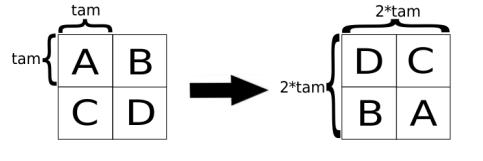
\includegraphics[width=300pt]{./recortar.jpg}
\end{center}
\end{figure}

Luego, comparamos la cantidad de ciclos producidos por $C$ y por $Assembler$.\newline

\subsection{Comparación de Tiempo}

En primer lugar, decidimos observar de qué manera afectaba el valor de $tam$ con respecto a la cantidad de ciclos para que las evaluaciones realizadas posteriormente no tuvieran en cuenta dicha variación.\newline

\begin{itemize}
\item{Al probar lena de 200x200 con una cantidad de 1000 iteraciones y un tam de 20, el tiempo obtenido fue el siguiente:\newline
\newline
\textbf{Ciclos C:}                 35471.988\newline
\vspace{0.15cm}
\textbf{Ciclos ASM:}               3082.194\newline
\textbf{Tiempo C:}                 35471988\newline
\textbf{Tiempo ASM:}               3082194\newline}


\item{Al probar lena de 200x200 con una cantidad de 1000 iteraciones y un tam de 100, el tiempo obtenido fue el siguiente:\newline
\newline
\textbf{Ciclos C:}                 455075.719\newline
\vspace{0.15cm}
\textbf{Ciclos ASM:}               20131.344\newline
\textbf{Tiempo C:}                 455075728\newline
\textbf{Tiempo ASM:}               20131345\newline}


\item{Al probar lena de 200x200 con una cantidad de 1000 iteraciones y un tam de 50, el tiempo obtenido fue el siguiente:\newline
\newline
\textbf{Ciclos C:}                 140342.594\newline
\vspace{0.15cm}
\textbf{Ciclos ASM:}               4661.547\newline
\textbf{Tiempo C:}                 140342599\newline
\textbf{Tiempo ASM:}               4661547\newline}

\item{Al probar lena de 200x200 con una cantidad de 1000 iteraciones y un tam de 150, el tiempo obtenido fue el siguiente:\newline
\newline
\textbf{Ciclos C:}                 1425689.625\newline
\vspace{0.15cm}
\textbf{Ciclos ASM:}               76169.781\newline
\textbf{Tiempo C:}                 1425689550\newline
\textbf{Tiempo ASM:}               76169781\newline}

\item{Al probar lena de 200x200 con una cantidad de 1000 iteraciones y un tam de 198, el tiempo obtenido fue el siguiente:\newline
\newline
\textbf{Ciclos C:}                 2665166.0\newline
\vspace{0.15cm}
\textbf{Ciclos ASM:}               127451.609\newline
\textbf{Tiempo C:}                 2665166175\newline
\textbf{Tiempo ASM:}               127451610\newline}


\begin{figure}[H] %[h] Aqui [b] para button [t] para top
\begin{center}
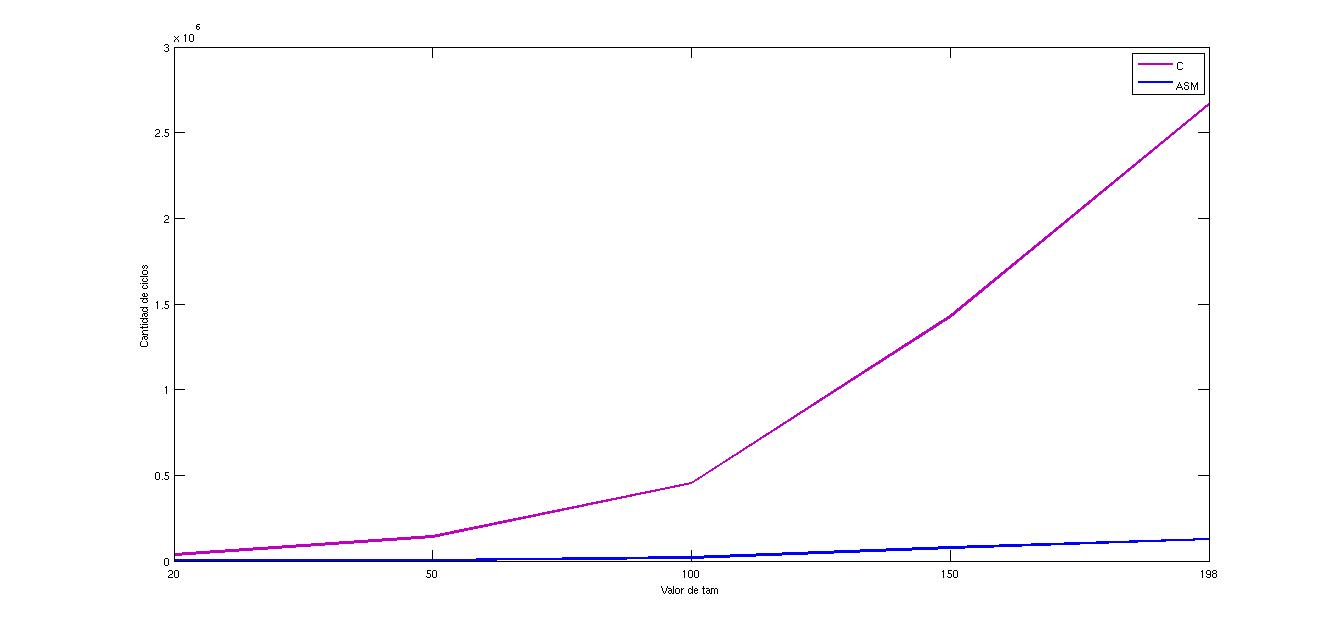
\includegraphics[width=560pt]{./variacionTam.jpg}
\end{center}
\end{figure}

A partir de dicha experimentación, podemos afirmar que el valor de $tam$ afecta de manera casi proporcional dado que a medida que $tam$ aumenta, la cantidad de iteraciones a realizar por el programa son mayores pues la cantidad de bits a copiar en la imagen destino es mayor. Luego, de manera tal a lograr enfocar el análisis en la cantidad de ciclos realizados de acuerdo al tamaño de la imagen, decidimos utilizar un $tam$ fijado en 100.\newline 

\item{Al probar lena de 200x200 con una cantidad de 10000 iteraciones y un tam de 100, el tiempo obtenido fue el siguiente:\newline
\newline
\textbf{Ciclos C:}                 788030.562\newline
\vspace{0.15cm}
\textbf{Ciclos ASM:}               11289.318\newline
\textbf{Tiempo C:}                 7880305902\newline
\textbf{Tiempo ASM:}               112893186\newline}

\item{Al probar lena de 204x204 con una cantidad de 10000 iteraciones y un tam de 100, el tiempo obtenido fue el siguiente:\newline
\newline
\textbf{Ciclos C:}                 790751.312\newline
\vspace{0.15cm}
\textbf{Ciclos ASM:}                9520.975\newline
\textbf{Tiempo C:}                 7907512983\newline
\textbf{Tiempo ASM:}               95209743\newline}

\item{Al probar lena de 256x256 con una cantidad de 10000 iteraciones y un tam de 100, el tiempo obtenido fue el siguiente:\newline
\newline
\textbf{Ciclos C:}                 794230.688\newline
\vspace{0.15cm}
\textbf{Ciclos ASM:}               13292.92\newline
\textbf{Tiempo C:}                 7942306884\newline
\textbf{Tiempo ASM:}               132929199\newline}


\item{Al probar lena de 512x512 con una cantidad de 10000 iteraciones y un tam de 100, el tiempo obtenido fue el siguiente:\newline
\newline
\textbf{Ciclos C:}                 883575.438\newline
\vspace{0.15cm}
\textbf{Ciclos ASM:}               17408.297\newline
\textbf{Tiempo C:}                 8835754415\newline
\textbf{Tiempo ASM:}               174082968\newline}


\item{Al probar lena de 1023x767 con una cantidad de 10000 iteraciones y un tam de 100, el tiempo obtenido fue el siguiente:\newline
\newline
\textbf{Ciclos C:}                  943862.688\newline
\vspace{0.15cm}
\textbf{Ciclos ASM:}               42174.125\newline
\textbf{Tiempo C:}                 9438626621\newline
\textbf{Tiempo ASM:}               421741242\newline}

\end{itemize}

\begin{figure}[H] %[h] Aqui [b] para button [t] para top
\begin{center}
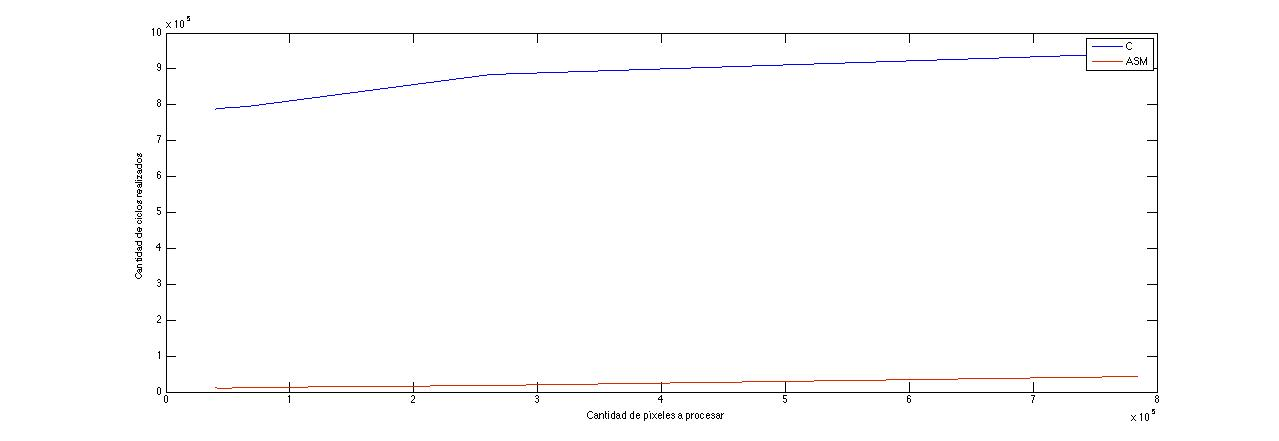
\includegraphics[width=560pt]{./ciclosRecortar.jpg}
\end{center}
\end{figure}

\item {\textbf{Halftone:}}
La idea principal de este filtro consistió en partir la imagen original en bloques de 2x2 píxeles generando, en la imagen destino, bloques del mismo tamaño. A cada nuevo bloque de la imagen original se le debió asignar el color blanco o negro dependiendo del valor de $t = \sum_{i=0}^{3} {(p_{i}}$, con $p_{i}$ píxeles del bloque de la imagen original de acuerdo a ciertas condiciones requeridas.\newline
Para la realización de dicho filtro, debimos almacenar en memoria valores que fueron necesarios durante la implementación. Éstos resultaron ser los valores con los que se compararía la sumatoria de los 4 bits como también un inversor (formado por 1's) y distinguidores entre la primer fila y la segunda (formados por 00ff y ff00 consecutivamente).\newline 
Por otro lado, fue necesario que tanto el ancho como el alto de la imagen fueran pares para poder iterar de a dos filas y columnas a la vez. Para ello, dividimos n y m por 2 y comparamos el resto con 0. En caso de serlo, m y n se mantenían. Caso contrario, se le restaba 1 a la variable impar.\newline
Luego, proseguimos recorriendo las matrices de fuente y destino. Para ello, decidimos desplazarnos a través de los punteros, por lo tanto, mientras estuviéramos en la misma fila, nos encargamos de sumarle 16 a rdi y a rsi en cada iteración. Al final de cada ciclo, el valor alcanzado por rsi y rdi era comparado con el ancho-16 para luego decidir si el ciclo debía continuar normalmente o si se había llegado al final de la fila. Una vez que el valor de rdi y rsi llegaban o superaban el ancho-16, se pasaba al final de la fila, donde rdi y rsi se seteaban en el ancho-16 para terminar procesando los últimos 16 bits. Para tratar la última columna, decidimos copiar el ciclo principal de manera tal a no tener que utilizar registros en exceso para determinar cuándo se debía pasar a la siguiente fila dado que no teníamos registros disponibles.\newline
Luego, dado que procesamos de a dos filas, debíamos desplazar nuestro puntero a rdi+16+row\_size+basura. Ésto se debe a que, en primer lugar, rdi terminaba la columna apuntando a ancho-16, luego era necesario sumar 16 para llegar al ancho. Por otro lado, se suma la basura para llegar al final de la fila de la imagen, por último, se suma el row\_size para saltear la fila siguiente. En el siguiente gráfico puede observarse la manera en la que se conforma una fila:\newline
\begin{figure}[H] %[h] Aqui [b] para button [t] para top
\begin{center}
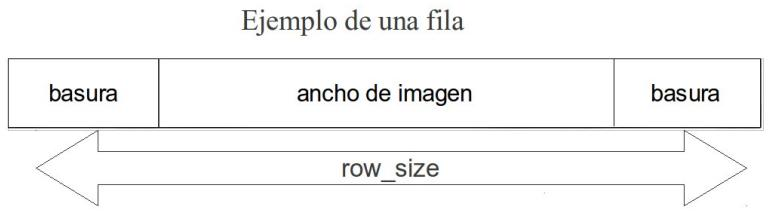
\includegraphics[width=300pt]{./fila.jpg}
\end{center}
\end{figure}
Para procesar los bits, nos encargamos de desempaquetamos de a dos filas. Luego, sumamos los píxeles dos a dos en cada fila. Finalmente, realizamos la suma de las posiciones de las filas correspondientes con las columnas correspondientes de la siguiente manera:\newline
\newline
Considerando la siguiente imagen,
\begin{figure}[H] %[h] Aqui [b] para button [t] para top
\begin{center}
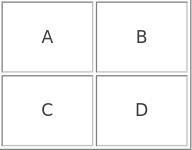
\includegraphics[width=90pt]{./suma.jpg}
\end{center}
\end{figure}
los pasos realizados fueron:\newline
- A+B\newline
- C+D\newline
- (A+B) + (C+D)\newline

Luego, se prosiguió realizando la comparación pcmpgtw entre la suma y los valores seteados para la comparación. Dado que el resultado deseado era el inverso ($\leq$ en vez de $>$), se aplicó un xor con el inversor a cada resultado obtenido por la comparación. Por último, se realizó un and entre lo obtenido de invertir la comparación y los filtrados de primera y segunda fila. Esta suma de operaciones debieron realizarse la cantidad de veces necesaria como para cubrir todos los valores con los que comparar la suma de píxeles. Luego, 4 veces. Por último, las máscaras fueron unidas con un 'or' en el que se juntaron las columnas respectivas de la primera y segunda fila. Los píxeles resultantes fueron, entonces, ubicados en la matriz destino.\newline
Los píxeles resultantes debían cumplir con la siguiente condición:
\begin{figure}[H] %[h] Aqui [b] para button [t] para top
\begin{center}
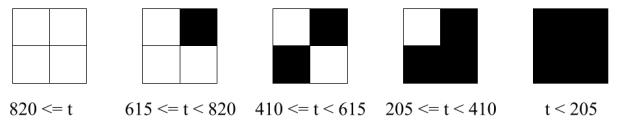
\includegraphics[width=400pt]{./halftone.jpg}
\end{center}
\end{figure}

\subsection{Comparación de Tiempo}

\begin{itemize}
\item{Al probar lena.bmp de 200x200, con una cantidad de 10000 iteraciones, el tiempo obtenido fue el siguiente:\newline
\newline
\textbf{Ciclos C:}                  517667.594\newline
\vspace{0.15cm}
\textbf{Ciclos ASM:}               32787.918\newline
\textbf{Tiempo C:}                 5176676016\newline
\textbf{Tiempo ASM:}               327879162\newline}

\item{Al probar lena.bmp de 204x204, con una cantidad de 10000 iteraciones, el tiempo obtenido fue el siguiente:\newline
\newline
\textbf{Ciclos C:}                 745335.375\newline
\vspace{0.15cm}
\textbf{Ciclos ASM:}               21178.518\newline
\textbf{Tiempo C:}                 7453353516\newline
\textbf{Tiempo ASM:}               211785186\newline}


\item{Al probar lena.bmp de 256x256, con una cantidad de 10000 iteraciones, el tiempo obtenido fue el siguiente:\newline
\newline
\textbf{Ciclos C:}                 1175849.5\newline
\vspace{0.15cm}
\textbf{Ciclos ASM:}               30366.938\newline
\textbf{Tiempo C:}                 11758494252\newline
\textbf{Tiempo ASM:}               303669366\newline}

\item{Al probar lena.bmp de 512x512, con una cantidad de 10000 iteraciones, el tiempo obtenido fue el siguiente:\newline
\newline
\textbf{Ciclos C:}                  3217938.0\newline
\vspace{0.15cm}
\textbf{Ciclos ASM:}               200020.438\newline
\textbf{Tiempo C:}                 32179380138\newline
\textbf{Tiempo ASM:}               2000204397\newline}

\item{Al probar lena.bmp de 1023x767, con una cantidad de 10000 iteraciones, el tiempo obtenido fue el siguiente:\newline
\newline
\textbf{Ciclos C:}                 13136558.0\newline
\vspace{0.15cm}
\textbf{Ciclos ASM:}               343688.281\newline
\textbf{Tiempo C:}                 131365579827\newline
\textbf{Tiempo ASM:}               3436882980\newline}

\end{itemize}

\begin{figure}[H] %[h] Aqui [b] para button [t] para top
\begin{center}
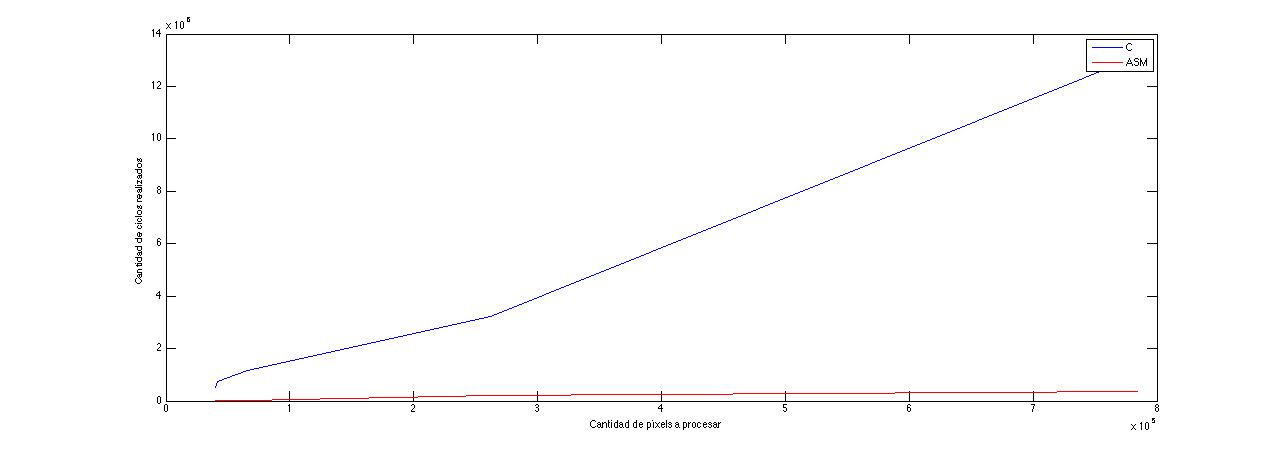
\includegraphics[width=560pt]{./ciclosHalftone.jpg}
\end{center}
\end{figure}

\item {\textbf{Umbralizar:}}
En Umbralizar, la imagen destino debía cumplir los siguientes requisitos:\newline
- Cada píxel menor a $min$ debía valer 0.\newline
- Cada píxel mayor a $max$ debía valer 255.\newline
- Caso contrario, el píxel debía valer $\lfloor p/Q \rfloor$.Q\newline
con $min$, $max$ y $Q$ enteros de 1 byte.\newline
\newline
Para lograr dicho objetivo, pasamos los valores $max$, $min$ y $Q$ (enteros) a floats para realizar los cálculos necesarios. Para ello, desempaquetamos y convertimos los píxeles a dicho tipo de dato.\newline
Nuestro ciclo consistió en procesar de a 16 bits comparando los píxeles con $max$ y $min$ con la operación pcmpgtw. Las máscaras resultantes fueron, luego, invertidas con 0xff00's dado que el resultado deseado era la comparación inversa a la facilitada por Intel. Luego, se debieron procesar los píxeles que no fueron menores a $min$ ni mayores a $max$. Para ello, se los dividió por $Q$, se los redondeó a parte entera con la función roundps y luego se los multiplicó nuevamente por $Q$. Por último, los convertimos a doubleword para luego empaquetar y terminar por juntar las máscaras con and y or y procesar los píxeles. Todo lo explicitado anteriormente fue realizado de manera rápida gracias al procedimiento realizado con SSE.\newline
Para recorrer la matriz, decidimos desplazarnos a través de los punteros, por lo tanto, mientras estuviéramos en la misma fila, nos encargamos de sumarle 16 a rdi y a rsi en cada iteración. Al final de cada ciclo, el valor alcanzado por rsi y rdi era comparado con el ancho-16 para luego decidir si el ciclo debía continuar normalmente o si se había llegado al final de la fila. Una vez que el valor de rdi y rsi llegaban o superaban el ancho-16, se pasaba al final de la fila, donde rdi y rsi se seteaban en el ancho-16 para terminar procesando los últimos 16 bits. Para tratar la última columna, decidimos copiar el ciclo principal de manera tal a no tener que utilizar registros en exceso para determinar cuándo se debía pasar a la siguiente fila dado que no teníamos registros disponibles.\newline
\subsection{Comparación de Tiempo}

\begin{itemize}
\item{Al probar lena.bmp de 200x200, con una cantidad de 10000 iteraciones y 64 128 16 como parámetros, el tiempo obtenido fue el siguiente: \newline
\newline
\textbf{Ciclos C:}                  1112498.0\newline
\vspace{0.15cm}
\textbf{Ciclos ASM:}               531874.0\newline
\textbf{Tiempo C:}                 11124979713\newline
\textbf{Tiempo ASM:}               5318740134\newline}

\item{Al probar lena.bmp de 204x204, con una cantidad de 10000 iteraciones y 64 128 16 como parámetros, el tiempo obtenido fue el siguiente: \newline
\newline
\textbf{Ciclos C:}                 1149053.75\newline
\vspace{0.15cm}
\textbf{Ciclos ASM:}               599925.562\newline
\textbf{Tiempo C:}                 11490536914\newline
\textbf{Tiempo ASM:}               5999255621\newline}

\item{Al probar lena.bmp de 256x256, con una cantidad de 10000 iteraciones y 64 128 16 como parámetros, el tiempo obtenido fue el siguiente: \newline
\newline
Ciclos C:                 1631805.5\newline
\vspace{0.15cm}
Ciclos ASM:               601924.359\newline
Tiempo C:                 16318054494\newline
Tiempo ASM:               6019243697\newline}

\item{Al probar lena.bmp de 512x512, con una cantidad de 10000 iteraciones y 64 128 16 como parámetros, el tiempo obtenido fue el siguiente: \newline
\newline
\textbf{Ciclos C:}                  6794335.0\newline
\vspace{0.15cm}
\textbf{Ciclos ASM:}               3372920.25\newline
\textbf{Tiempo C:}                 67943348235\newline
\textbf{Tiempo ASM:}               33729202260\newline}

\item{Al probar lena.bmp de 1023x767, con una cantidad de 10000 iteraciones y 64 128 16 como parámetros, el tiempo obtenido fue el siguiente: \newline
\newline
\textbf{Ciclos C:}                  6794335.0\newline
\vspace{0.15cm}
\textbf{Ciclos ASM:}               3372920.25\newline
\textbf{Tiempo C:}                 67943348235\newline
\textbf{Tiempo ASM:}               33729202260\newline}

\end{itemize}

\begin{figure}[H] %[h] Aqui [b] para button [t] para top
\begin{center}
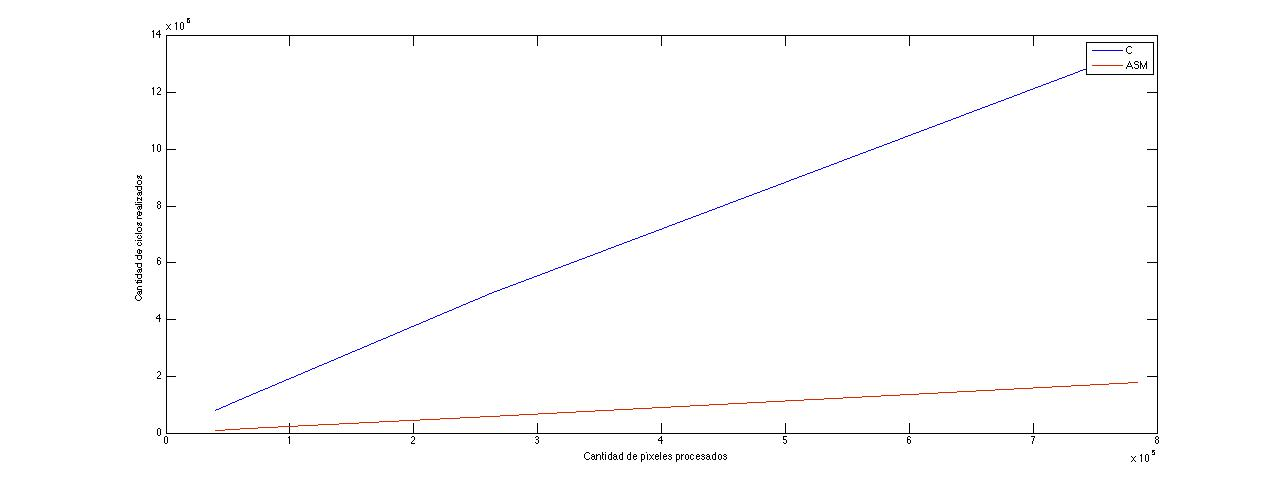
\includegraphics[width=560pt]{./ciclosUmbralizar.jpg}
\end{center}
\end{figure}

\item {\textbf{Colorizar:}}
Para colorizar, la imagen fuente debía ser procesada de acuerdo a las siguientes definiciones: 

\begin{figure}[H] %[h] Aqui [b] para button [t] para top
\begin{center}
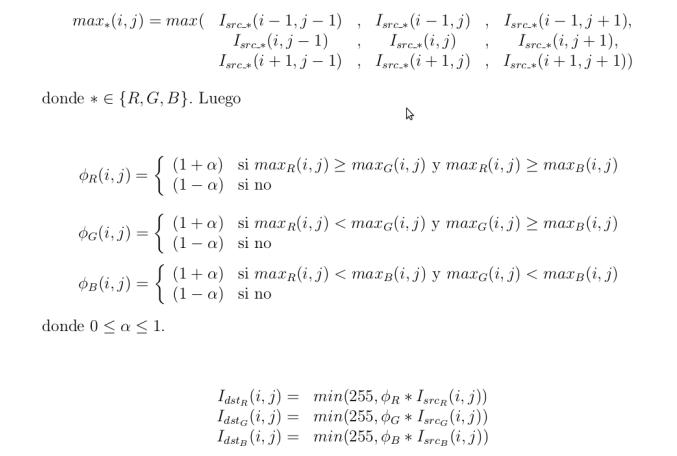
\includegraphics[width=400pt]{./colorizar.jpg}
\end{center}
\end{figure}

Para ello, decidimos procesar nuestra matriz de la siguiente forma:\newline
En primer lugar, pasamos el ancho de píxeles a bytes multiplicándolo por 3. Para iterar las filas, le restamos 2 al ancho pues éstas eran procesadas de a 3. Luego, nos creamos 3 contadores para desplazarnos de manera tal a evitar modificar los punteros rdi y rsi originales en cada columna. Cada contador correspondía a una fila distinta. El resto de la matriz fue recorrida de la misma manera mencionada en los filtros anteriores.\newline
Para procesar la primera y última fila y columna, nos limitamos a copiar los píxeles de fuente y pegarlos en destino. Para el resto de las filas, optamos por levantar tramos de 3x5 píxeles y quedarnos con la fila del medio (de las 3 procesadas). Luego, comparamos fila con fila para sacar el máximo de cada canal en dicha columna. Continuamos desplazando los registros de modo que quedaran las columnas alineadas con el fin de calcular los máximos de cada grupo de píxeles. Más tarde, calculamos los máximos y obtuvimos 3 píxeles de los máximos valores. El procedimiento sería el siguiente:\newline
\newline
Tramo de 3x5 píxeles(el último byte es descarte):\newline
		(0 1 2)(3 4 5)(6 7 8)(9 10 11)(12 13 14)(15\newline
		(0 1 2)(3 4 5)(6 7 8)(9 10 11)(12 13 14)(15\newline
		(0 1 2)(3 4 5)(6 7 8)(9 10 11)(12 13 14)(15\newline
\newline
Desplazamiento de los registros de modo para lograr columnas alineadas para calcular los máximos de cada grupo de píxeles:\newline
		.\hspace{2cm}(0 1 2)(3  4  5)(6  7  8)(9 10 11)(12\newline
		(0 1 2)(3 4 5)(6  7  8)(9 10 11)(12 13 14)(15\newline
		(3 4 5)(6 7 8)(9 10 11)(12 13 14)(15 xx xx)(xx\newline
		
Obtención luego del cálculo de los máximos: 3 píxeles con los máximos valores:\newline
		(x x x)(3 4 5)(6  7  8)(9 10 11)(xx xx xx)(xx\newline
\newline
Luego, continuamos viendo qué canal era el máximo para duplicar sus píxeles y comparar los 3 canales (por canales nos referimos a R, G y B) de cada uno. Proseguimos descartando el primer byte para que quedara alineado al desempaquetar. Nuestro resultado quedó, entonces de la siguiente manera:\newline
		x x)(3 4 5)(6  7  8)( 9 10 11)(xx xx xx)(xx xx\newline
		\newline
Nuestra implementación continuó con el desempaquetamiento los canales. Luego, proseguimos cargando las máscaras y filtrándos los canales de manera tal a quedar con el rojo por un lado, el verde por otro y por último el azul. A partir de aquí, pudimos realizar las comparaciones necesarias para el máximo de los canales en la parte alta y parte baja. A partir de estas comparaciones, nos generamos las máscaras necesarias que acomodamos para que respetaran el siguiente orden: 0 0 0 B G R B G R B G R 0 0 0 0.\newline
Por último, desempaquetamos los datos originales y los filtros para realizar los cálculos correspondientes: multiplicación de los phi por el canal correspondiente y terminar por truncar a int y empaquetar nuevamente los datos para escribir.
\subsection{Comparación de Tiempo}

\begin{itemize}
\item{Al probar lena.bmp de 200x200, con una cantidad de 10000 iteraciones y 0.5 como parámetro, el tiempo obtenido fue el siguiente:\newline
\newline
\textbf{Ciclos C:}                 14686647.0\newline
\vspace{0.15cm}
\textbf{Ciclos ASM:}               512187.438\newline
\textbf{Tiempo C:}                  146866477084\newline
\textbf{Tiempo ASM:}               5121874249\newline}

\item{Al probar lena.bmp de 204x204, con una cantidad de 10000 iteraciones y 0.5 como parámetro, el tiempo obtenido fue el siguiente:\newline
\newline
\textbf{Ciclos C:}                 15266872.0\newline
\vspace{0.15cm}
\textbf{Ciclos ASM:}               538598.312\newline
\textbf{Tiempo C:}                 152668724208\newline
\textbf{Tiempo ASM:}               5385982752\newline}

\item{Al probar lena.bmp de 256x256, con una cantidad de 10000 iteraciones y 0.5 como parámetro, el tiempo obtenido fue el siguiente:\newline
\newline
\textbf{Ciclos C:}                 24220022.0\newline
\vspace{0.15cm}
\textbf{Ciclos ASM:}               1257442.375\newline
\textbf{Tiempo C:}                 242200208670\newline
\textbf{Tiempo ASM:}               12574423775\newline}

\item{Al probar lena.bmp de 512x512, con una cantidad de 10000 iteraciones y 0.5 como parámetro, el tiempo obtenido fue el siguiente:\newline
\newline
\textbf{Ciclos C:}                 95509400.0\newline
\vspace{0.15cm}
\textbf{Ciclos ASM:}               5063423.0\newline
\textbf{Tiempo C:}                 955094000358\newline
\textbf{Tiempo ASM:}               50634231520\newline}

\item{Al probar lena.bmp de 1023x767, con una cantidad de 10000 iteraciones y 0.5 como parámetro, el tiempo obtenido fue el siguiente:\newline
\newline
\textbf{Ciclos C:}                 280806784.0\newline
\vspace{0.15cm}
\textbf{Ciclos ASM:}               15221196.0\newline
\textbf{Tiempo C:}                 2808067870590\newline
\textbf{Tiempo ASM:}               152211957569\newline}

\end{itemize}

\begin{figure}[H] %[h] Aqui [b] para button [t] para top
\begin{center}
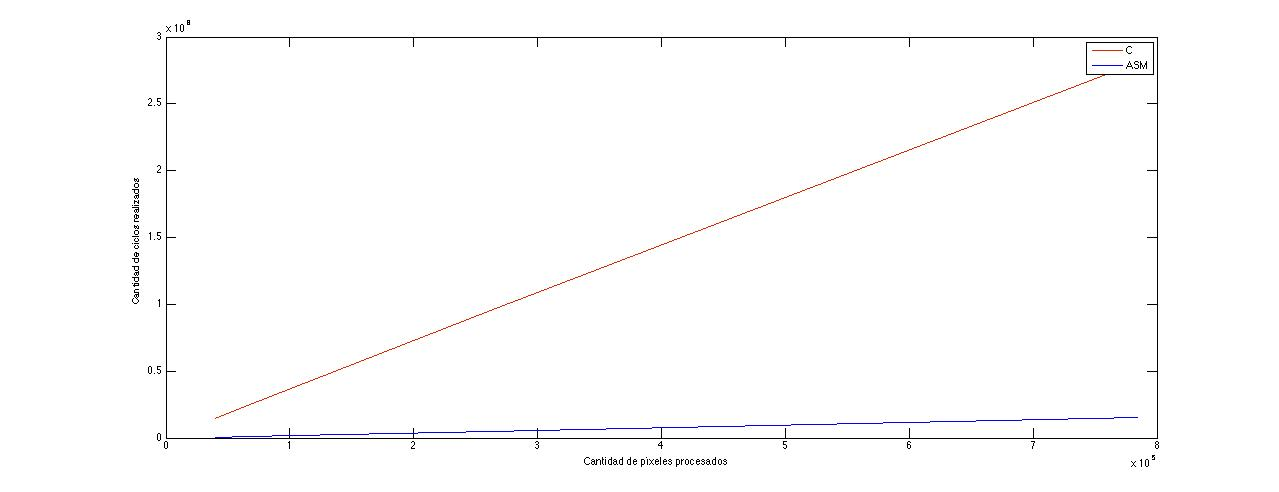
\includegraphics[width=560pt]{./ciclosColorizar.jpg}
\end{center}
\end{figure}

\item {\textbf{Waves:}}
La idea de Waves consistió en combinar la imagen fuente con una imagen de ondas dando tonos más oscuros y más claros en forma de onda. Éstas se generan de manera repetida a lo largo de los ejes x e y. Cada píxel $(i,j)$ de la imagen destino se obtuvo a través del siguiente cálculo:
\begin{figure}[H] %[h] Aqui [b] para button [t] para top
\begin{center}
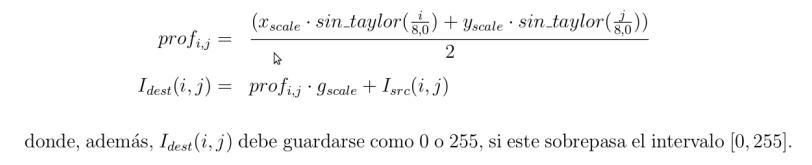
\includegraphics[width=400pt]{./prof.jpg}
\end{center}
\end{figure}

La función waves requiere la utilización de $sin\_taylor(x)$ que cumple con el siguiente pseudocódigo:
\begin{figure}[H] %[h] Aqui [b] para button [t] para top
\begin{center}
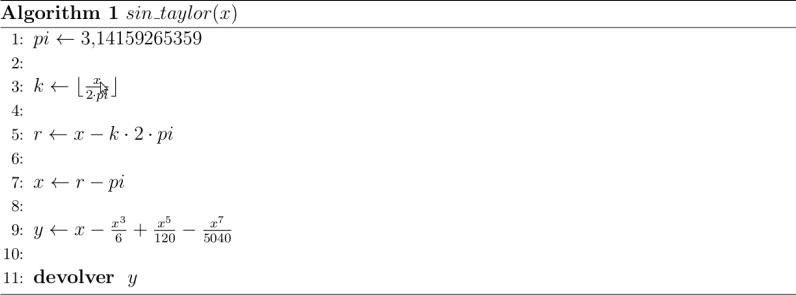
\includegraphics[width=400pt]{./algoritmo_waves.jpg}
\end{center}
\end{figure}
Para la implementación de dicho filtro, calculamos el $sin\_taylor$ siguiendo los pasos del pseudocódigo. Para ello, almacenamos los valores necesarios en memoria en floats, por ejemplo $\pi$ empaquetado, los índices para las columnas y los valores necesarios para operar con el $sin\_taylor$. Para no hacer llamados a memoria dentro del ciclo, nos limitamos a almacenar dichos valores en registros de uso general. De este modo, ahorramos tiempo de ejecución. Por otro lado, para realizar los cálculos, utilizamos las instrucciones de SSE necesarias para manipular enteros (para calcular k) y floats (el resto de las variables). Para realizar la potencia, debimos multiplicar la cantidad de veces necesaria dado que no encontramos una operación que realizara dicho procedimiento. Vale aclarar que, para lograr una mayor claridad, decidimos respetar el orden seguido por el pseudocódigo.\newline
Para procesar cada fila, realizamos un call a $sin\_taylor$ y, con el fin de calcular la profundidad en un tiempo razonable, se preparó un arreglo con cuatro valores del 0 al 3 que serían usados como índice de columna para dicho cálculo. Por otra parte, se preparó un arreglo de 0's para la realización del cálculo del seno de la fila. Este procedimiento se realizó 4 veces hasta llegar al píxel número 16.\newline
Luego, proseguimos desempaquetando a doublewords y convirtiendólos a floats para multiplicar a prof por el píxel debido para terminar empaquetando a bytes.\newline
Para recorrer la matriz, recorrimos las filas hasta el ancho-16. Una vez alcanzado o superado ese valor, restamos el valor del que se pasó de ancho-16 y procesamos la última columna copiando el ciclo anterior. Una vez alcanzada la última columna, la función se dio por terminada.
\subsection{Comparación de Tiempo}

\begin{itemize}
\item{Al probar lena.bmp de 200x200, con una cantidad de 10000 iteraciones y 2.0 4.0 16.0 como parámetros, el tiempo obtenido fue el siguiente:\newline
\newline
\textbf{Ciclos C:}                  85787504.0\newline
\vspace{0.15cm}
\textbf{Ciclos ASM:}               869124.625\newline
\textbf{Tiempo C:}                 857875015971\newline
\textbf{Tiempo ASM:}               8691245955\newline}

\item{Al probar lena.bmp de 204x204, con una cantidad de 10000 iteraciones y 2.0 4.0 16.0 como parámetros, el tiempo obtenido fue el siguiente:\newline
\newline
\textbf{Ciclos C:}                 63717420.0\newline
\vspace{0.15cm}
\textbf{Ciclos ASM:}               831478.375\newline
\textbf{Tiempo C:}                 637174228992\newline
\textbf{Tiempo ASM:}               8314783716\newline}

\item{Al probar lena.bmp de 256x256, con una cantidad de 10000 iteraciones y 2.0 4.0 16.0 como parámetros, el tiempo obtenido fue el siguiente:\newline
\newline
\textbf{Ciclos C:}                 100537464.0\newline
\vspace{0.15cm}
\textbf{Ciclos ASM:}               1297188.5\newline
\textbf{Tiempo C:}                 1005374601537\newline
\textbf{Tiempo ASM:}               12971885286\newline}


\item{Al probar lena.bmp de 512x512, con una cantidad de 10000 iteraciones y 2.0 4.0 16.0 como parámetros, el tiempo obtenido fue el siguiente:\newline
\newline
\textbf{Ciclos C:}                  540099392.0\newline
\vspace{0.15cm}
\textbf{Ciclos ASM:}               5443293.0\newline
\textbf{Tiempo C:}                 5400993944457\newline
\textbf{Tiempo ASM:}               54432932814\newline}


\item{Al probar lena.bmp de 1023x767, con una cantidad de 10000 iteraciones y 2.0 4.0 16.0 como parámetros, el tiempo obtenido fue el siguiente:\newline
\newline
\textbf{Ciclos C:}                  1618532352.0\newline
\vspace{0.15cm}
\textbf{Ciclos ASM:}               16243114.0\newline
\textbf{Tiempo C:}                 16185323663982\newline
\textbf{Tiempo ASM:}               162431140968\newline}

\end{itemize}

\begin{figure}[H] %[h] Aqui [b] para button [t] para top
\begin{center}
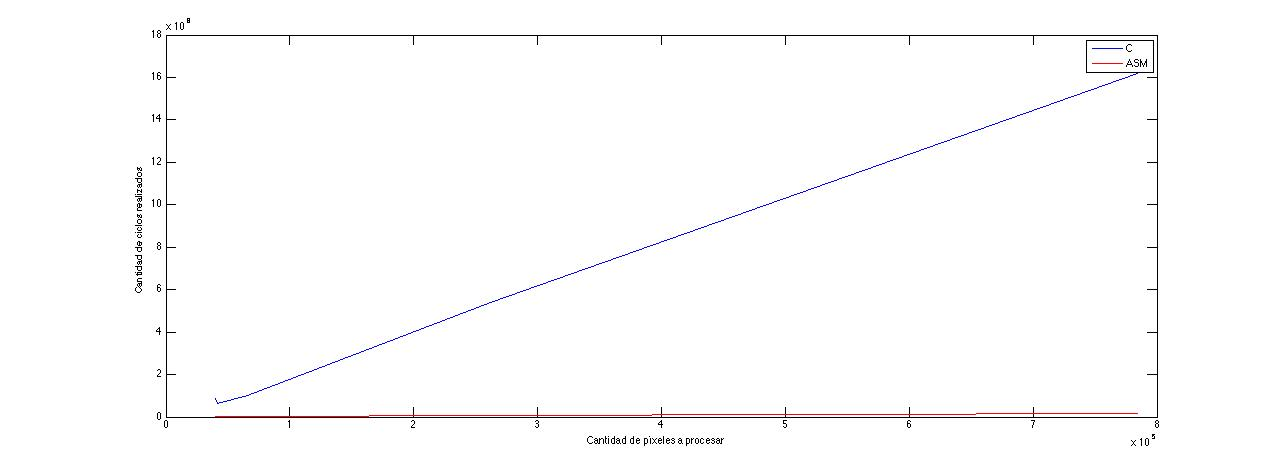
\includegraphics[width=560pt]{./ciclosWaves.jpg}
\end{center}
\end{figure}

\item {\textbf{Rotar:}} 
El filtro rotar toma la imagen de entrada y escribe en la de salida la imagen rotada 45 grados. Cada píxel de la imagen resultante se forma de la siguiente manera:
\begin{figure}[H] %[h] Aqui [b] para button [t] para top
\begin{center}
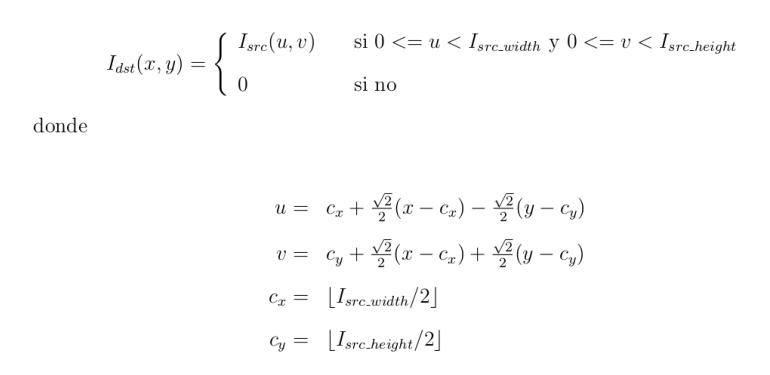
\includegraphics[width=400pt]{./rotar.jpg}
\end{center}
\end{figure}
El filtro rotar no es un buen candidato para paralelizar. Esto se debe a que, al levantar los píxeles consecutivos de la imagen fuente, éstos no deben ser consecutivos en la imagen destino. Esto significa que el orden de los píxeles de la imagen destino es distinto al de la imagen fuente. Nuestra manera de paralelizar fue al realizar los cálculos que le darían la posición correcta a la imagen destino.\newline
Luego del análisis previo, elegimos proceder de la siguiente manera:\newline
En primer lugar, calculamos Cy y Cx con simples shr del ancho y alto de la imagen fuente. Luego, procedimos calculando $\sqrt{2}$/2 habiendo extendido los cálculos a todos los bits del XMM para, luego, realizar los cálculos con todos los píxeles levantados en una iteración.\newline
Para realizar los cálculos tomando el índice $x$ correcto, decidimos almacenar una escalera en memoria de manera tal a evitar ciclos innecesarios y a realizar cuentas velozmente.\newline
Luego, procedimos realizando los cálculos necesarios para hallar $u$ y $v$. Una vez encontrados dichos valores, obtuvimos máscaras como resultado de las comparaciones que nos explicitarían dónde ubicar los píxeles en la imagen destino.\newline
El paso siguiente consistió en levantar cada píxel procesado dentro del arreglo y ubicarlo en su lugar correspondiente de salida de acuerdo a los offsets obtenidos. Dicho procedimiento fue realizado cuatro veces ya que cada arreglo almacenaba cuatro píxeles. De esta manera, todos los píxeles fueron procesados correctamente y de una manera más eficiente que si hubiésemos procesado bit a bit.\newline
Por último, para recorrer la matriz, decidimos utilizar un contador que le sumaríamos a rdi y a rsi de manera tal a no perder el puntero original. El resto de la ejecución se realizó del mismo modo que se describió anteriormente.\newline
Para la realización de dicho filtro, preferimos utilizar floats ya que para usar doubles debíamos desempaquetar una mayor cantidad de veces, utilizar más registros, complicar el código y demorar la ejecución de los ciclos. Si bien los doubles generan mayor precisión, el tipo de datos utilizado no impidió visualizar la imagen de manera clara por lo que nos decidimos por esa opción.

\subsection{Comparación de Tiempo}

\begin{itemize}

\item{Al probar lena.bmp de 200x200, con una cantidad de 10000 iteraciones, el tiempo obtenido fue el siguiente:\newline
\newline
\textbf{Ciclos C:}                  1741106.375\newline
\vspace{0.15cm}
\textbf{Ciclos ASM:}               654910.312\newline
\textbf{Tiempo C:}                 17411062968\newline
\textbf{Tiempo ASM:}               6549102981\newline}

\item{Al probar lena.bmp de 204x204, con una cantidad de 10000 iteraciones, el tiempo obtenido fue el siguiente:\newline
\newline
\textbf{Ciclos C:}                 1764135.5\newline
\vspace{0.15cm}
\textbf{Ciclos ASM:}               517955.594\newline
\textbf{Tiempo C:}                 17641354566\newline
\textbf{Tiempo ASM:}               5179556052\newline}

\item{Al probar lena.bmp de 256x256, con una cantidad de 10000 iteraciones, el tiempo obtenido fue el siguiente:\newline
\newline
\textbf{Ciclos C:}                 2711875.5\newline
\vspace{0.15cm}
\textbf{Ciclos ASM:}                790127.688\newline
\textbf{Tiempo C:}                27118754190\newline
\textbf{Tiempo ASM:}                7901277300\newline}


\item{Al probar lena.bmp de 512x512, con una cantidad de 1000 iteraciones, el tiempo obtenido fue el siguiente:\newline
\newline
\textbf{Ciclos C:}                 11218906.0\newline
\vspace{0.15cm}
\textbf{Ciclos ASM:}               3205361.25\newline
\textbf{Tiempo C:}                 112189065366\newline
\textbf{Tiempo ASM:}               32053613385\newline}
\end{itemize}
\end{itemize}

\begin{figure}[H] %[h] Aqui [b] para button [t] para top
\begin{center}
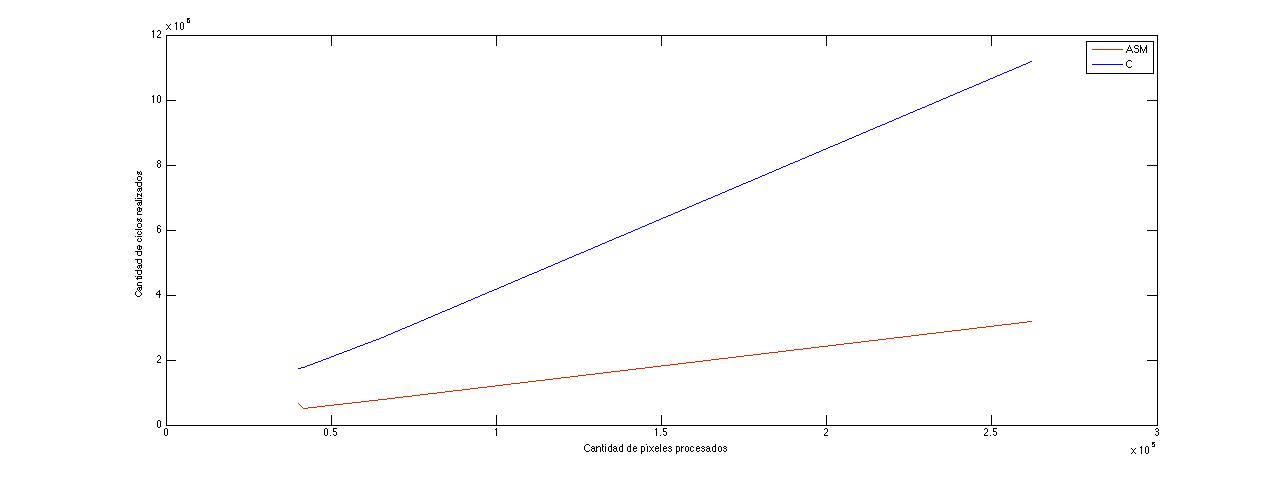
\includegraphics[width=560pt]{./ciclosRotar.jpg}
\end{center}
\end{figure}

\section{Resultados}
A partir de los valores obtenidos luego de varias pruebas realizadas para calcular el tiempo de ejecución de cada función $C$ y $Assembler$, pudimos concluir que cuanto mayor es el tamaño de la imagen a procesar, mayor es la cantidad de ciclos realizados por el programa como también el tiempo para procesarlos. Esto resulta lógico considerando que a mayor tamaño de imagen, más importante va a ser la cantidad de datos a procesar lo que implica que el tiempo de ejecución del programa sea más elevado.\newline
Luego de dichas conclusiones, decidimos utilizar objdump para lograr dar una explicación a lo obtenido:\newline
En primera instancia, hallamos que la cantidad de ciclos realizados por $Assembler$ es muy menor a la realizada por $C$. Esto se debe a que el $Assembler$ de $C$ realiza múltiples llamados a memoria en cada ciclo. Por ejemplo, la mayoría de los datos que utiliza son almacenados en la pila por lo que en cada iteración realiza operaciones utilizando, por ejemplo, [rbp-0x28]. Ésta es la causa principal del retraso temporal generado por el $C$ respecto del $Assembler$. \newline 
Por otro lado, nos resultó sorprendente la extensión de los códigos en $Assembler$ generados por los $C$ en comparación con los nuestros. Para hallarle una explicación a dicha consecuencia, pensamos que el causante de esto fue que, al estar todo almacenado en la pila, los desplazamientos requieren de numerosas instrucciones. Contrariamente, al moverse con un puntero, lo único necesario para el desplazamiento no es más que un incrementador. \newline
Por otra parte, hallamos que los códigos en $Assembler$ generados por los $C$ realizan operaciones innecesarias, como por ejemplo multiplicar por 1, dado que se producen de manera automática.\newline
Por último, encontramos que el ensamblado del $C$ no utiliza instrucciones SIMD, empaquetando y desempaquetando, por lo que la cantidad de operaciones a realizar está multiplicada por 16.\newline
En el siguiente gráfico, puede observarse el porcentaje sobre la cantidad de ciclos realizados por cada filtro en ASM a partir de los realizados por los mismos en C. En éste, puede verse claramente que la ejecución en C utiliza una cantidad de ciclos muy superior a los realizados por ASM:\newline
\begin{figure}[H] %[h] Aqui [b] para button [t] para top
\begin{center}
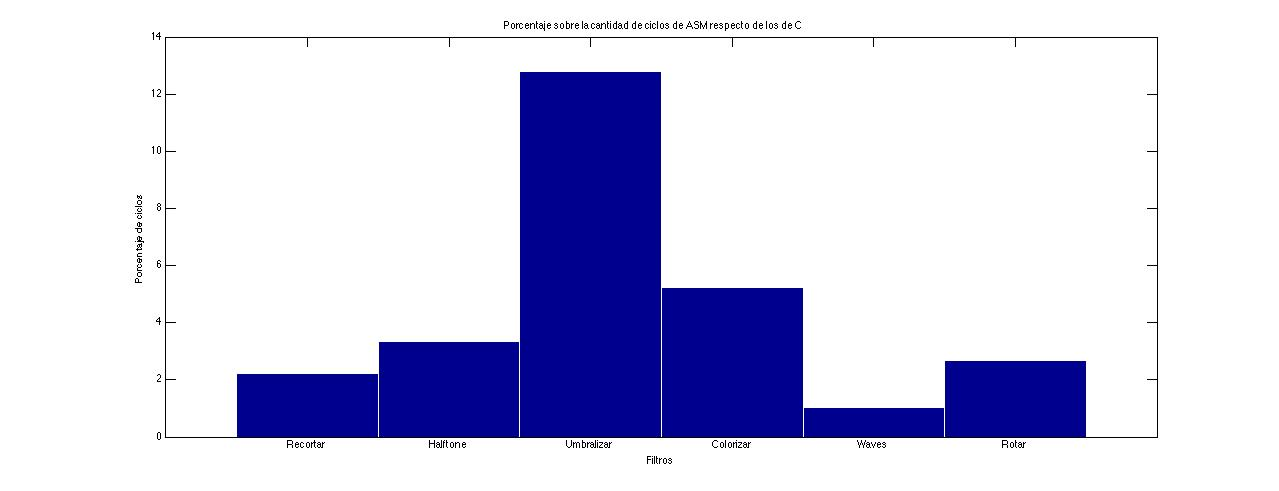
\includegraphics[width=570pt]{./velocidad.jpg}
\end{center}
\end{figure}
\section{Conclusi\'on}
Podemos concluir que las causas principales de que el código en $C$ sea mucho más lento que el código $Assembler$ dado que su ensamblado no utiliza instrucciones SIMD y almacena todos los datos en la pila que son llamados en cada iteración. Esto significa que $C$ usa la FPU que es poco performante causando un aumento del tiempo de ejecución.\newline
A partir de aquí, podemos afirmar que realizar operaciones de a muchos bits a la vez, empaquetando y desempaquetando los datos, acelera enormemente la ejecución de una función. Del mismo modo, los llamados a memoria dentro de los ciclos disminuyen la velocidad de ejecución excesivamente.

\end{document}
